\chapter{Digitalizace a zpracování signálů}

Výstupem samo-vyvažovacího můstku jsou dva harmonické signály 
reprezentující napětí a proud na měřeném obvodu. 
Tyto signály je potřeba zdigitalizovat a následně zpracovat tak, aby bylo následně možné vypočítat impedanci obvodu.

Pro výpočet komplexní impedance je potřeba znát amplitudy (nebo efektivní hodnoty) a fázový posun mezi oběma signály.
Dále je v tomto případě cílem měřit i střední hodnotu napětí, protože signály mohou mít stejnosměrnou složku.

Nezáleží, zda je měřena amplituda nebo efektivní hodnota napětí, protože důležité nejsou absolutní hodnoty napětí, ale jejich poměr.

\section{Metoda převodu na stejnosměrná napětí}

Jako nejjednodušší řešení se nabízí vytvořit obvod, 
který jednotlivé veličiny převede na stejnosměrné napětí, které je následně změřeno \acs{A/D} převodníkem (\acs{ADC}).

Výhodou takového přístupu je nízký nárok na vzorkovací rychlost ADC, které proto může být velmi precizní.
S tím se spojuje i jednoduchost zpracování v mikrokontroléru, který počítá pouze s několika vzorky.

Zásadním problémem je však náchylnost na šum, což se zejména projevuje při vyšších frekvencích.
Z toho důvodu se tato metoda v komerčních zařízeních nepoužívá.

\subsection{Špičkový detektor}
Pro měření amplitudy střídavého signálu lze použít špičkový detektor, který je realizován
kondenzátorem nabíjeným přes diodu, která bránjí vybíjení v závěrném směru.

Jak je ukázáno na schématu v obr. \ref{fig:sch_detector}, operační zesilovač v zapojení \uv{sledovač} se zpětnou vazbou zapojenou za diodu kompenzuje její propustné napětí.
Po odečtení hodnoty je špičkový detektor resetován tranzistorem, který zkratem vybije kondenzátor.
Poté je detektor připraven na další měření. \cite{elliott_peakdetection}

\begin{figure}[h!]
    \centering
    \includegraphics[width=0.45\textwidth]{obrazky/peak_detector_sch.pdf} % Adjusted width for a single figure
    \caption{Schéma špičkového detektoru}
    \label{fig:sch_detector} % Changed label for the first figure
\end{figure}

Špičkový detektor je citlivý na šum a jiné nežádoucí napěťové špičky v signálu, 
které mohou posunout naměřenou hodnotu výše, než je pravá hodnota signálu bez šumu.
Tento jev je je ukázán na grafu v obr. \ref{fig:chart_peakdetect}.
Čím delší je doba měření, tím větší je pravděpodobná nepřesnost.

\begin{figure}[h!]
    \centering
    \includegraphics[width=0.65\textwidth]{obrazky/peak_detect_chart.pdf} % Adjusted width for the second figure
    \caption{Graf vstupního a výstupního napětí šp. detektoru s demonstrací efektu šumu}
    \label{fig:chart_peakdetect} % Changed label for the second figure
\end{figure}

\subsection{Fázový detektor}
Fázový posun signálů může být měřen fázovými detektory fungujícími na principu průchodu nulou. Jednoduchá implementace takového 
detektoru je založena na logickém hradle XOR, do kterého vstupují pulzní signály z komparátorů, které indikují momentální
polaritu signálu \vizobr{fig:sch_XOR}.

Pokud mají signály stejnou fázi, mají v každý okamžik i stejnou polaritu, 
tudíž výstup XOR hradla 
nebude nikdy aktivní.
V případě opačné fáze signálů ($\varphi = 180^\circ$) je jejich polarita vždy
opačná, výstup XOR tedy bude aktivní 100\% času.

Při fázových posunech mezi těmito extrémy $\varphi\in(0^\circ;180^\circ)$ je střída výstupu XOR přímo úměrná 
fázovému posunu. Pro získání stejnosměrného napětí se použije RC filtr dolní propust,
který ze signálu získá střední hodnotu \vizobr{fig:chart_XOR}. \cite{ArtOfElectronics}

Fázový posun se ze střední hodnoty vypočítá následovně:
$$k = \frac{180}{U_{log}}$$
$$\varphi = k \cdot U_{XOR - stř} \quad [^\circ]$$


\begin{figure}[h!]
    \centering
    \includegraphics[width=0.65\textwidth]{obrazky/XOR_phase_sch.pdf} % Adjusted width for the second figure
    \caption{Schéma XOR fázového detektoru. \cite{ArtOfElectronics}}
    \label{fig:sch_XOR} % Changed label for the second figure
\end{figure}

\begin{figure}[h!]
    \centering
    \includegraphics[width=0.8\textwidth]{obrazky/XOR_phase_chart.pdf} % Adjusted width for the second figure
    \caption{Graf napětí XOR fázového detektoru.}
    \label{fig:chart_XOR} % Changed label for the second figure
\end{figure}

Měření fáze podle průchodu nulou je sice jednoduché, ale má nedostatky, které
brání použití pro přesné měřiče.

Jelikož logické hradlo XOR pracuje na logických úrovních, není zaručeno, že se jeho výstupní
napětí bude pohybovat mezi napájecím napětím a nulou. Odchylky ve výstupním napětí ovlivní 
výslednou vyfiltrovanou střední hodnotu.

Další problém je zapříčiněn možnou přítomností šumu na měřeném signálu.
Může se tedy stát, že v jedné půlperiodě signál projde nulou vícekrát, nebo že bude průchod nulou 
časově posunutý důsledkem fázového šumu na měřeném signálu. 
Graficky je tento fenomén zobrazen na obr. \ref{fig:chart_zerocross}.

\begin{figure}[h!]
    \centering
    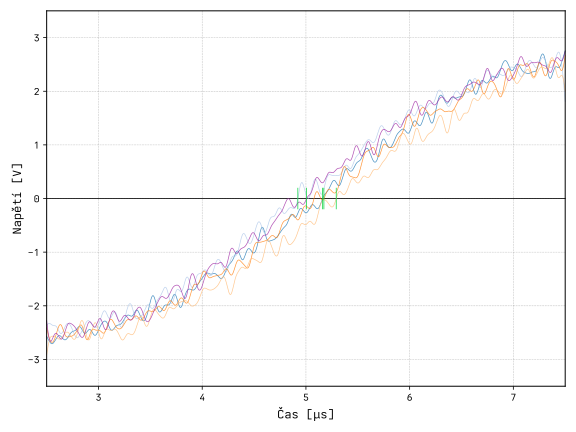
\includegraphics[width=0.8\textwidth]{obrazky/zerocross_noise_chart.pdf} % Adjusted width for the second figure
    \caption{Graf nepřesnosti detekce průchodu nulou způsobené šumem}
    \label{fig:chart_zerocross} % Changed label for the second figure
\end{figure}


\section{Metoda vzorkování a digitálního zpracování}

